\documentclass{article}
\usepackage[utf8]{inputenc}
\usepackage[spanish]{babel}
\usepackage[usenames,dvipsnames, table]{xcolor}
\usepackage{epsfig}
\usepackage{float}
\usepackage{hyperref}
\usepackage{subfig}
\usepackage{enumitem}
\usepackage{listings}
\usepackage{placeins}
\usepackage{import}

\usepackage{color}
\definecolor{gray}{rgb}{0.4,0.4,0.4}
\definecolor{darkblue}{rgb}{0.0,0.0,0.6}
\definecolor{cyan}{rgb}{0.0,0.6,0.6}

\lstset{
  basicstyle=\ttfamily,
  columns=fullflexible,
  showstringspaces=false,
  commentstyle=\color{gray}\upshape
}

\lstdefinelanguage{XML}
{
  morestring=[b]",
  morestring=[s]{>}{<},
  morecomment=[s]{<?}{?>},
  stringstyle=\color{black},
  identifierstyle=\color{darkblue},
  keywordstyle=\color{cyan},
  morekeywords={xmlns,version,type}
}

\hypersetup{%
  colorlinks=true,%
  linkcolor=blue,%
  citecolor=blue,%
  unicode%
}

\makeatletter
\newcommand{\logo}[2] {%
	\def\input@path{{#1}}
	\def\logoimg{#2}
}
\newcommand\version[1]{\renewcommand\@version{#1}}
\newcommand\@version{\@latex@error{No \noexpand\version given}\@ehc}
\makeatother

\graphicspath{{resources/}}

\begin{document}

\version{ @LATEX_VERSION@ }
\title{Testplatform}
\import{@CONFIG_PATH@/doxygen/}{title.tex}
\tableofcontents
\pagebreak

\section{Introducción}
Testplatform es una herramienta de línea de comandos interactiva que permite verificar el correcto funcionamiento de las APIs de la plataforma. Para ello se hace uso de una batería de tests cuyo resultado deberá ser comprobado por el usuario.

\FloatBarrier

\section{Tests de las APIs}
Cada API posee un test y cada uno de éstos está dividido en pasos, los cuales prueban de manera atómica cada una de las funcionalidades provistas. Cuando un paso comienza, se muestra su nombre y una breve descripción del mismo \textit{(ver Figura~\ref{fig:test_description})}, para luego proseguir con la prueba. Existen dos tipos de pasos, aquellos automáticos, cuyo resultado es determinado por la herramienta, y los manuales, cuyo resultado es determinado por el usuario mediante el uso de las \hyperref[sec:control_keys]{teclas de control}; en la Figura~\ref{fig:accept_result} se muestra como el paso solicita la elección del resultado. Además, dentro de los pasos manuales, existe un subconjunto de pasos que requieren que el usuario realice algún tipo de acción extra; cuando este sea el caso, el paso imprimirá en la consola las instrucciones a seguir \textit{(ver Figura~\ref{fig:test_instructions})}.

\begin{figure}[h]
\centering
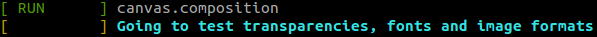
\includegraphics[scale=0.50]{testdescription}
\caption{Descripción del paso canvas.composition}
\label{fig:test_description}
\end{figure}

\begin{figure}[h]
\centering
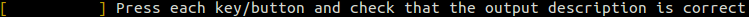
\includegraphics[scale=0.50]{testinstructions}
\caption{Instrucciones del paso input.map}
\label{fig:test_instructions}
\end{figure}

\begin{figure}[h]
\centering
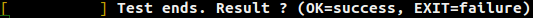
\includegraphics[scale=0.50]{testaccept}
\caption{Selección de resultado de la prueba}
\label{fig:accept_result}
\end{figure}

En la sección~\ref{sec:tests} se presentará cada test de manera detallada e individual.

\FloatBarrier

\section{Resultados}
Cuando un paso termine, se mostrará cual ha sido su resultado mediante un mensaje en la consola, este puede ser ``FAILED'' \textit{(ver Figura~\ref{fig:test_failed})}, en caso de falla, ``OK'' \textit{(ver Figura~\ref{fig:test_successful})}, en caso de éxito, o ``SKIPPED'' \textit{(ver Figura~\ref{fig:test_skipped})} si hubiera sido obviado mediante las~\hyperref[sec:control_keys]{teclas de control}.

\begin{figure}[h]
\centering
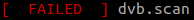
\includegraphics[scale=0.50]{testfailed}
\caption{Resultado de un paso que ha fallado}
\label{fig:test_failed}
\end{figure}
\FloatBarrier
\begin{figure}[h]
\centering

\includegraphics[scale=0.50]{testok}
\caption{Resultado de un paso exitoso}
\label{fig:test_successful}
\end{figure}
\FloatBarrier
\begin{figure}[h]
\centering
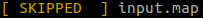
\includegraphics[scale=0.50]{testskipped}
\caption{Paso salteado}
\label{fig:test_skipped}
\end{figure}

\FloatBarrier

Al finalizar todos los tests que hayan sido ejecutados se mostrará el resultado de la prueba, detallando:

\begin{itemize}
	\item Cantidad de tests corridos.
	\item Cantidad de pasos corridos.
	\item Cantidad de pasos exitosos.
	\item Cantidad de pasos salteados.
	\item Cantidad de pasos fallidos.
\end{itemize}

En caso de haber pasos fallidos se listará el nombre junto con la descripción de cada uno de los mismos.
La Figura~\ref{fig:results} muestra como son visualizados los resultados obtenidos luego de la ejecución de los tests.

\begin{figure}[h!]
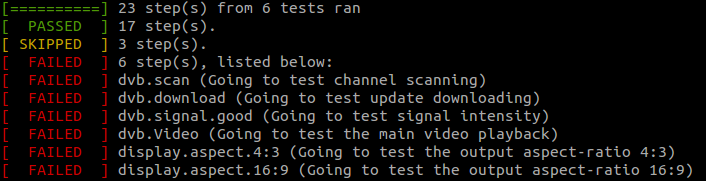
\includegraphics[scale=0.50]{testresults}
\caption{Resultados de la prueba}
\label{fig:results}
\end{figure}

\FloatBarrier

\section{Teclas de control}
\label{sec:control_keys}
Las teclas de control son teclas que tienen una función determinada durante el transcurso de la ejecución de la herramienta, existen dos tipos de teclas de control, las que se utilizan para determinar el resultado de un paso; y las de navegación. Las primeras son las teclas OK y EXIT, que establecen que el paso que acaba de finalizar ha sido exitoso o no, respectivamente. 
Las teclas de navegación sirven para desplazarse entre los tests y/o pasos, las mismas son:

\begin{itemize}
	\item Flecha hacía arriba: Navega hacía el test siguiente.
	\item Flecha hacía abajo: Navega hacía el test anterior.
	\item Flecha hacía la derecha: Navega hacía el paso siguiente.
	\item Flecha hacía la izquierda: Repite el paso actual sí es que éste terminó, caso contrario navega hacía el paso anterior. Un paso ha terminado cuándo imprime en pantalla la leyenda ``Test ends'' y se encuentra en espera de que el usuario determine su resultado.
\end{itemize}

\section{Tests paso a paso}
\label{sec:tests}

\subsection{Input}
\label{sec:input_test}

%01
\subsubsection{input.map}
Prueba que la asociación de las teclas sea correcta y completa. Cada vez que se presione alguna tecla se mostrará su nombre en la consola \textit{(ver Figura~\ref{fig:console})}.\\
Nota: Se puede presionar cualquier tecla con excepción de las \hyperref[sec:control_keys]{teclas de control}.

\begin{figure}[h]
\centering
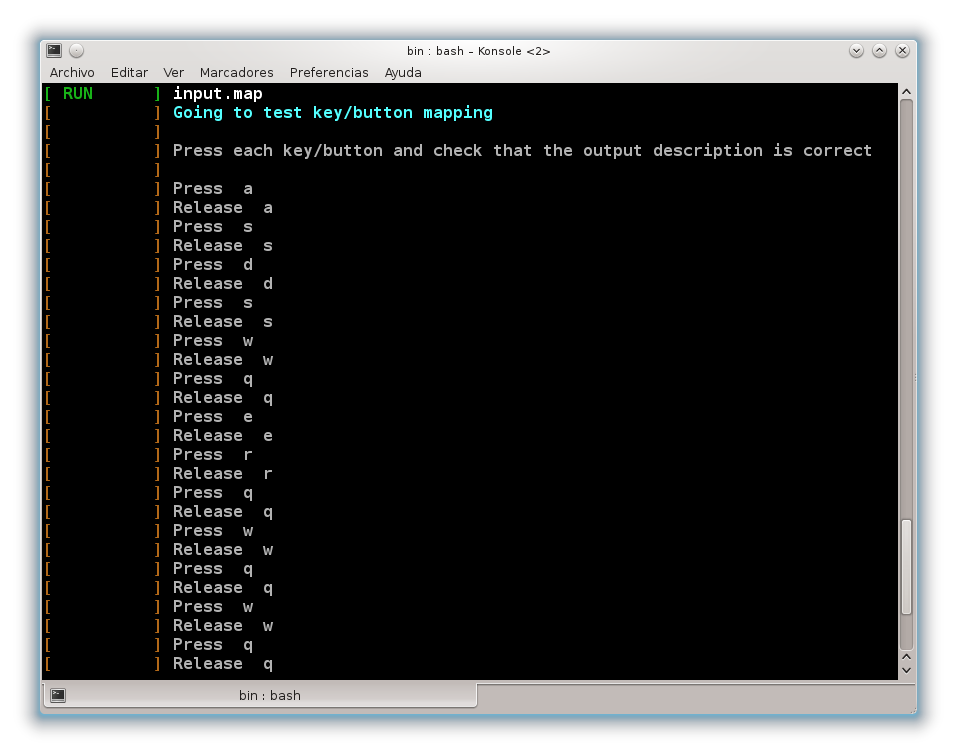
\includegraphics[scale=0.45]{keys}
\caption{Consola durante la ejecución del paso input.map}
\label{fig:console}
\end{figure}

\FloatBarrier
\subsection{Canvas}
\label{sec:canvas_test}

%02
\subsubsection{canvas.composition}
Prueba la transparencia en superficies, la correctitud de las tipografías. Para llevar a cabo ésta prueba se dibuja en pantalla:
\begin{itemize}
	\item Tres cuadrados semitransparentes que se suporponen entre sí.
	\item Texto con las fuentes Tiresias y DejaVuSans, ambas en todas sus variantes (normal, bold, italic y bold-italic).
\end{itemize}
El resultado final del paso deberá ser el exhibido en la Figura~\ref{fig:canvas_composite}

\begin{figure}[h]
\centering
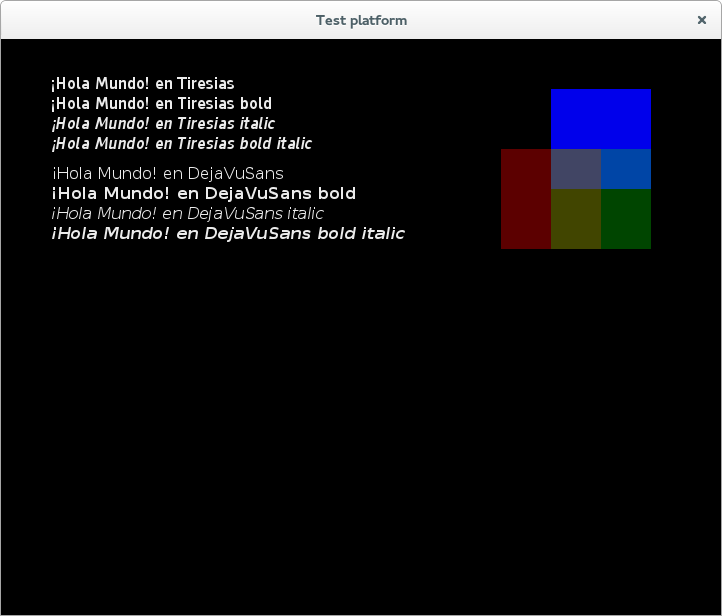
\includegraphics[scale=0.45]{composite}
\caption{Test canvas.composite}
\label{fig:canvas_composite}
\end{figure}

\FloatBarrier

\subsubsection{canvas.format}
Prueba el soporte para el dibujado de imagenes en distintos formatos. Los formatos a probar deben ser configurados. Consulte la sección \ref{sec:conf} para mas detalles.

%03
\subsection{Mediaplayer}
\label{sec:mediaplayer_test}

\FloatBarrier
\subsubsection{mediaplayer.format}
Prueba la reproducción de distintos formatos de archivos de tipo media, tanto video como sonido. Para indicar los formatos a probar consultar la sección~\ref{sec:conf}

\FloatBarrier
%04
\subsubsection{mediaplayer.volume}
\label{sec:mediaplayer_volume}
Reproduce un sonido; el volumen es colocado en 0 y luego es incrementado cada \texttt{X} segundos en un porcentaje \texttt{Y} hasta llegar al máximo.
\texttt{X} e \texttt{Y} son valores configurables, siendo \texttt{X} igual a la variable \texttt{volumeDuration} e \texttt{Y} igual a la variable \texttt{volumeStep}. Los valores por defecto de las variables son detallados en la sección~\ref{sec:conf}.

\FloatBarrier
%05
\subsubsection{mediaplayer.resize}
Reproduce un video en pantalla completa, pasados 2 segundos el video es redimensionado para ocupar la mitad de su tamaño original, siendo el resultado esperado el mostrado en la Figura~\ref{fig:mediaplayer_resize}

\begin{figure}[h]
\centering
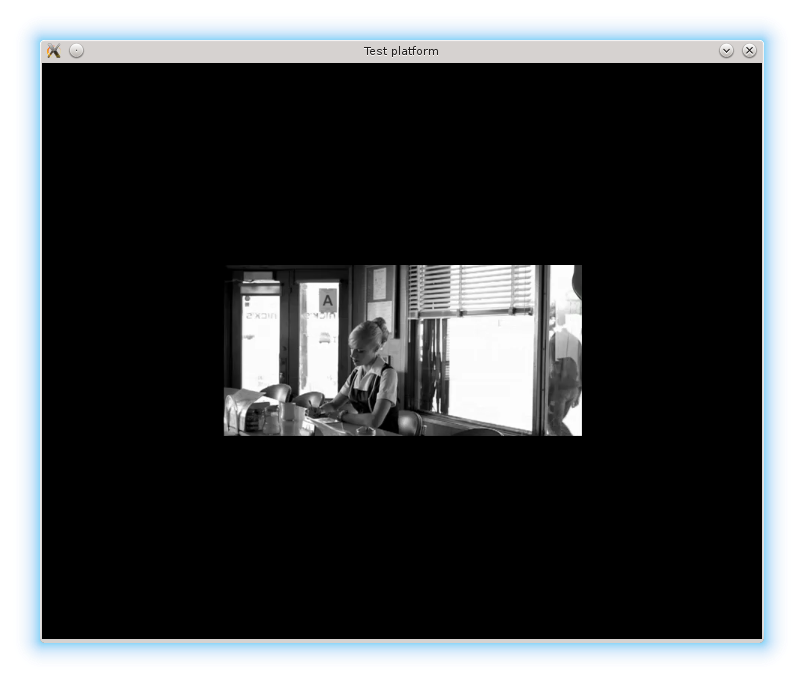
\includegraphics[scale=0.45]{resize_mediaplayer}
\caption{Video redimensionado}
\label{fig:mediaplayer_resize}
\end{figure}

\FloatBarrier

\subsection{Mixer}
\label{sec:mixer_test}

\FloatBarrier

%06
\subsubsection{mixer.volume}
\label{sec:mixer_volume}
Reproduce un sonido; el volumen del canal maestro del mixer es colocado en 0 y luego es incrementado cada \texttt{X} segundos en un porcentaje \texttt{Y} hasta llegar al máximo.
\texttt{X} e \texttt{Y} son valores configurables, siendo \texttt{X} igual a la variable \texttt{volumeDuration} e \texttt{Y} igual a la variable \texttt{volumeStep}. Los valores por defecto de las variables son detallados en la sección~\ref{sec:conf}.

\FloatBarrier

%07
\subsubsection{mixer.output.mono}
Reproduce un sonido mientras que la salida de audio está en modo mono.

\FloatBarrier

%08
\subsubsection{mixer.output.estereo}
Reproduce un sonido mientras que la salida de audio está en modo estéreo.

\FloatBarrier

%09
\subsubsection{mixer.mute}
Reproduce un sonido, éste no debe ser escuchado dado que el canal maestro del mixer está en modo mudo.

\FloatBarrier

%10
\subsubsection{mixer.unmute}
Reproduce un sonido, éste debe ser escuchado dado que el canal maestro del mixer no está en modo mudo.

\FloatBarrier

\subsection{DVB}
\label{sec:dvb_test}

\FloatBarrier

%11
\subsubsection{dvb.scan}
Verifica el correcto funcionamiento del escaneo de frecuencias, para ello se espera encontrar servicios específicos los cuales son parte del \textit{transport stream} de prueba. La información sobre el \textit{transport stream} es presentada en la sección~\ref{sec:ts}.\\
Nota: De ser encontrados los servicios esperados el test pasará exitosamente de manera automática

\FloatBarrier

%12
\subsubsection{dvb.download}
Comprueba el correcto funcionamiento de la descarga de actualizaciones, intentando hacerlo desde un servicio específico que es parte del \textit{transport stream} de prueba.\\
Nota: De lograrse descargar la actualización exitosamente el test pasará de manera automática.

\FloatBarrier

%13
\subsubsection{dvb.signal.bad}
Prueba la detección de la intensidad de la señal; en éste test se espera que la señal sea pobre, por lo cual es necesario que antes de confirmar su ejecución la antena esté desconectada.\\
Nota: Si la intensidad de la señal es mala el test pasará exitosamente de manera automática.

\FloatBarrier

%14
\subsubsection{dvb.signal.good}
Prueba la detección de la intensidad de la señal; en éste test se espera que la señal sea buena, por lo cual es necesario que antes de confirmar su ejecución la antena esté conectada.\\
Nota: Si la intensidad de la señal es buena el test pasará exitosamente de manera automática.

\FloatBarrier

%15
\subsubsection{dvb.video}
Prueba el video principal reproduciéndolo durante dos segundos en pantalla completa, para luego redimensionarlo a la mitad de su tamaño original, siendo el resultado esperado el de la Figura~\ref{fig:dvb_video_resize}.

\begin{figure}[h]
\centering
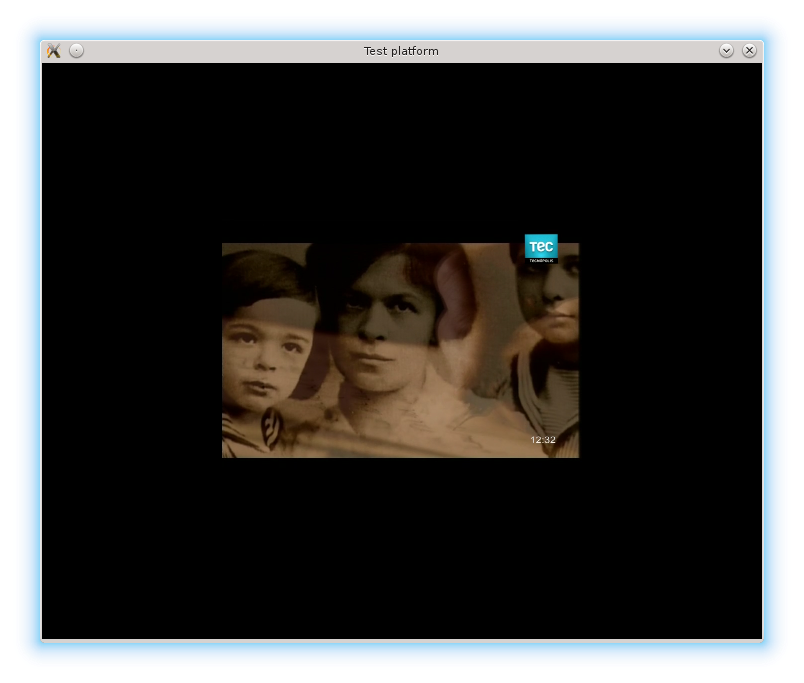
\includegraphics[scale=0.45]{resize_video}
\caption{Video principal redimensionado}
\label{fig:dvb_video_resize}
\end{figure}

\FloatBarrier

\subsection{Display}
\label{sec:display_test}

\FloatBarrier

%16
\subsubsection{display.aspect.4:3}
Prueba el cambio a la relación de aspecto 4:3 del dispositivo.

\FloatBarrier

%17
\subsubsection{display.aspect.16:9}
Prueba el cambio a la relación de aspecto 16:9 del dispositivo.

\FloatBarrier

%18
\subsubsection{display.mode}
Prueba el cambio de resoluciones y/o salidas de video en el dispositivo. Las resoluciones y salidas probadas son configurables. Consulte la sección \ref{sec:conf} para mas detalles.

\FloatBarrier

\section{Configuración}
\label{sec:conf}
La herramienta brinda la posibilidad de ser configurada a través de archivos xml, los mismos definen valores de variables que son utilizadas para brindar más flexibilidad durante la ejecución de los tests. Existen dos tipos de configuraciones posibles:

\subsection{Configuración general}

\begin{description}
  \item[volumeDuration:] Duración del nivel de volumen. Su valor por defecto es de dos segundos.
  \item[volumeStep:] Incremento en el nivel de volumen por cada iteración, está definido como un porcentaje. Su valor por defecto es 25\%.
\end{description}

Un ejemplo de archivo de configuración general es mostrado en la Figura \ref{fig:general_conf_file}

\begin{figure}[h]
\centering
\begin{lstlisting}[language=xml]
<?xml version="1.0" encoding="UTF-16" standalone="no" ?>
<root>
  <tool>
    <testplatform>
      <volumeDuration>1</volumeDuration>
      <volumeStep>10</volumeStep>
    </testplatform>
  </tool>
</root>
\end{lstlisting}
\caption{Archivo de configuración general}
\label{fig:general_conf_file}
\end{figure}

\subsection{Configuración de los tests}
Este tipo de configuración se utiliza para indicarle a la herramienta ciertos parámetros de los tests. Los archivos que pueden ser utilizados son:

\begin{description}
  \item[canvas.imageformats.xml:] Configura los formatos de imagenes a probar.
  \item[mediaplayer.formats.sound.xml:] Configura los formatos de sonidos a probar.
  \item[mediaplayer.formats.video.xml:] Configura los formatos de video a probar.
  \item[display.connectors.composite.xml:] Configura los modos a probar para las salida de video composite.
  \item[display.connectors.component.xml:] Configura los modos a probar para las salida de video component.
  \item[display.connectors.hdmi.xml:] Configura los modos a probar para las salida de video hdmi.
  \item[display.connectors.vga.xml:] Configura los modos a probar para las salida de video vga.
  \item[display.connectors.svideo.xml:] Configura los modos a probar para las salida de video svideo.
  \item[display.connectors.dvi.xml:] Configura los modos a probar para las salida de video dvi.
\end{description}

Un ejemplo de archivo de configuración para canvas.imageformats.xml es mostrado en la Figura \ref{fig:test_conf_file}

\begin{figure}[h]
\centering
\begin{lstlisting}[language=xml]
<?xml version="1.0" encoding="UTF-16" standalone="no" ?>
<?xml version="1.0" encoding="UTF-8" standalone="yes" ?>
<root>
  <Items>
    <item>bmp</item>
    <item>jpg</item>
    <item>jp2</item>
    <item>png</item>
    <item>gif</item>
    <item>tiff</item>
  </Items>
</root>
\end{lstlisting}
\caption{Archivo de configuración}
\label{fig:conf_file}
\end{figure}

\FloatBarrier

\section{Opciones de la herramienta}
La herramienta acepta opciones mediante la línea de comandos, algunas de las opciones aceptadas son:
\begin{itemize}
\item --help: Muestra la ayuda
\item --tests=args: Define los tests a correr, si no se específica correrán todos. \\
\textit{args} es un conjunto de nombres de tests separados por una coma.
Los tests disponibles son:

\begin{itemize}
  \item input
  \item canvas
  \item display
  \item mediaplayer
  \item dvb
  \item mixer
\end{itemize}
Ejemplo: ``--test=canvas,mixer,dvb''.
\end{itemize}

Para ver otras opciones utilice el comando -h o --help.

\FloatBarrier

\section{Caracteristicas del transport stream de prueba}
\label{sec:ts}
El \textit{transport stream} a transmitir debe estar compuesto por dos servicios con las siguientes características:\\

Primer servicio:

\begin{itemize}
\setlength{\itemindent}{.20in}
	\item Nombre del servicio: ``SD - Prueba OTA''.
	\item Número de servicio: 0xf1a0.
	\item Debe contener una actualización de firmware.
\end{itemize}

Segundo servicio:

\begin{itemize}
\setlength{\itemindent}{.20in}
	\item Nombre del servicio: ``HD - Prueba OTA''.
	\item Número de servicio: 0xf1a1.
	\item No debe contener actualizaciones de firmware.
\end{itemize}

Es necesario transmitirlos para el correcto funcionamiento de los tests de dvb.

\FloatBarrier

\end{document}
